\documentclass[a4paper,10pt]{article}

\usepackage{ifpdf}
\ifpdf
  \usepackage[pdftex]{graphicx}
  \graphicspath{{images/}}
\else
  \RequirePackage[dvipdfm, CJKbookmarks, bookmarks=true, bookmarksnumbered=true%
                unicode,%
             colorlinks,%
         citecolor=blue,%
             hyperindex,%
       plainpages=false,%
      pdfstartview=FitH]{hyperref}
  \AtBeginDvi{\special{pdf:tounicode UTF8-UCS2}}
  \usepackage[dvipdfm]{graphicx}
  \graphicspath{{images/}}
  \DeclareGraphicsExtensions{.eps}
\fi

%\RequirePackage{CJKutf8,CJKnumb,CJKulem}
\RequirePackage{CJKutf8,CJKnumb}
\RequirePackage{color,verbatim,cite}
\RequirePackage{texnames,makeidx,indentfirst}
\RequirePackage{amsmath,amssymb,amsfonts,bm,manfnt}
\RequirePackage{fancyhdr,titlesec,datetime}
\RequirePackage{wasysym,longtable,multirow,bigstrut}
\usepackage[section]{placeins}
\usepackage[left=3.2cm,right=2.54cm,top=3.3cm,bottom=2.6cm]{geometry}
\usepackage[caption=false,font=footnotesize]{subfig}

\AtBeginDocument{\begin{CJK*}{UTF8}{song}\CJKtilde\CJKindent\CJKcaption{utf8}}
\AtEndDocument{\end{CJK*}}

\setlength{\parskip}{0.75ex plus .2ex minus .5ex}
\renewcommand{\baselinestretch}{1.2}

\hypersetup {
    pdftitle={无线传感器网络中的位置相关安全研究},
    pdfauthor={杨文博}
}

\title{无线传感器网络中的位置相关安全研究}
\author{杨文博}

\begin{document}

\maketitle

\section{ 选题依据 } 

\subsection{课题的研究意义和国内外研究的概况}

\subsubsection{无线传感器网络及其中的安全问题}  

无线传感器网络(Wireless Sensor Network, WSN)在最近几年获得了全球的广泛关注。伴随着与传感器相关的通信、嵌入式和分布式计算技术的飞速发展,特别是微机电系统(Micro-Electro-Mechanical, MEMS)的长足进步,人们研制出了各种不同共用的廉价微型传感器。这些传感器可以感知、测量并收集所处的环境信息,并将这些信息通过某种方式传输给布置~WSN~的用户。它们可以被广泛应用于国防军事、国家安全、环境监测、火灾预警、交通管理、医疗卫生和灾难救援等许多领域,帮助人们获得大量有价值的目标环境信息。

无线传感器节点一般情况下由感应模块、处理器、内存、能量供应、无线模块和控制单元组成。装配着不同的感应模块的传感器可以感应物理环境的不同信息,例如湿度、温度、压力、震动、风速、声音、辐射、有毒气体含量等等。由于其廉价性和微型化,无线传感器所采用的处理器一般比较低端,不支持如浮点运算、多媒体指令等一些高级功能。无线传感器节点一般都只有少量的内存,它所收集到的信息将使用无线方式传输到基站。一般情况下,无线传感器节点的能源主要由电池供应,后备能源可以根据环境的不同采用太阳能等其它的能量供应方式。

无线传感器网络则是由大量无线传感器节点构成的分布式、自组织的无线网络。典型的无线传感器网络一般由数十到数千个无线传感器节点组成,用来检测一定范围区域内的环境信息。受无线传感器节点体积小、数量大、资源受限的限制,~WSN~往往具有以下特点:

\begin{enumerate}

\item 树形路由、多跳转发。WSN~需要将收集到的信息传回基站,所以一般构成以基站为根节点的树形结构;由于信号的覆盖范围受限,无线传感器节点间通信往往需要经过多跳转发,其转发由传感器节点完成,没有专门的路由设备。

\item 无线传输的带宽、稳定性和安全性较差。由于底层采用无线通信,受到信道本身物理特性的限制,~WSN~的通信质量和稳定性往往较差;考虑到无线信号的开放性,其更容易受到信道窃听、伪装、拒绝服务等攻击,需要特别考虑一些安全需求。

\item 网络资源受限。~WSN~中,无线节点往往不具有长期的电源供应,节点设计的计算能力、存储空间都要比一般的有线网络节点要小得多。在设计网络网络结构时需要特别考虑到能耗因素,避免部分节点能源耗尽导致整个网络失灵。

\end{enumerate}

\begin{figure}[htbp]
  \centering
  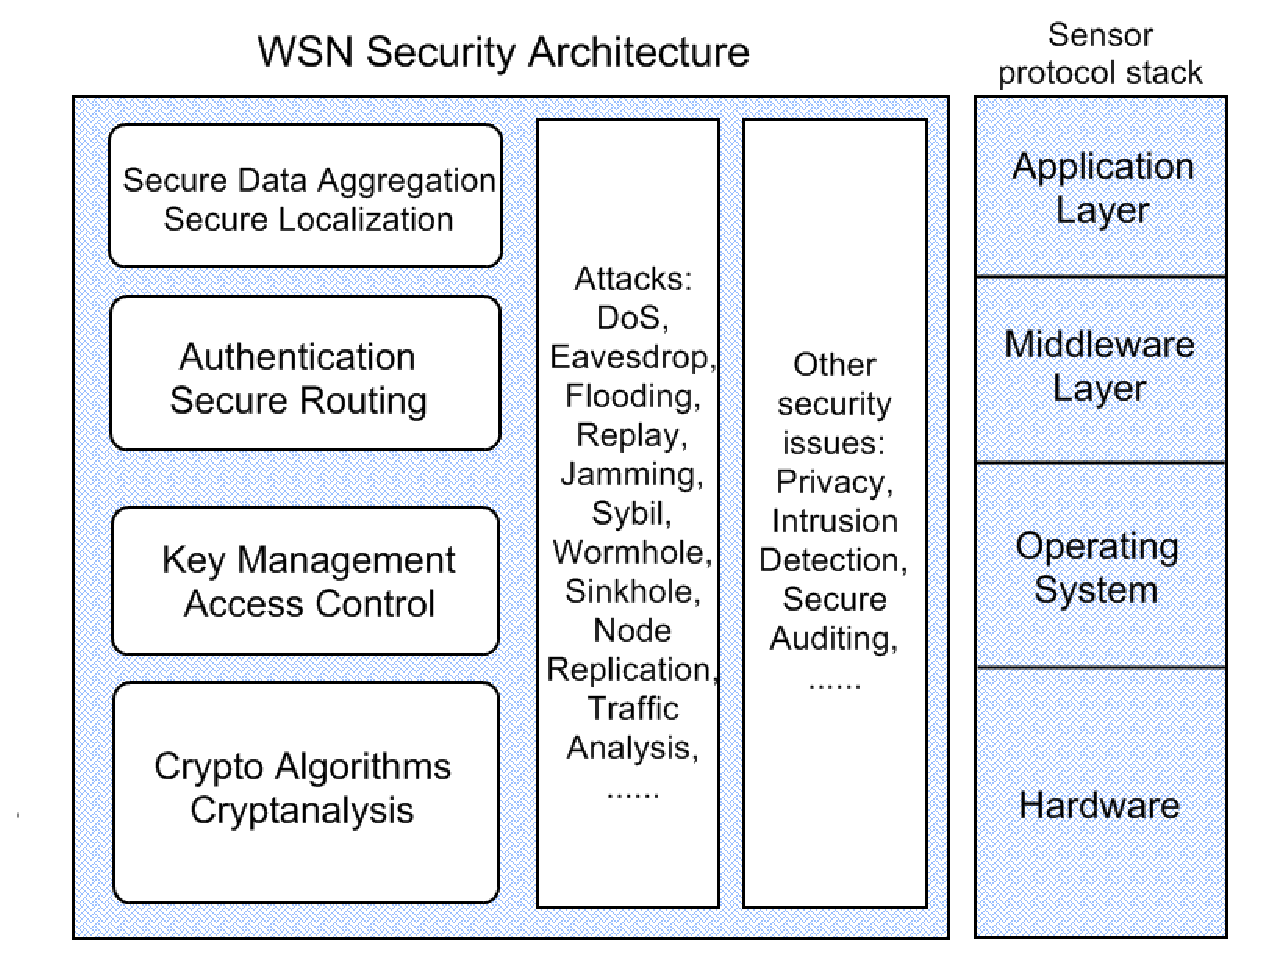
\includegraphics[width=0.8\textwidth,keepaspectratio]{wsn_sec_map}
  \caption{\label{wsn_sec_map}~WSN~安全架构~\cite{Li2005}}
\end{figure}

由于受以上条件限制,很多传统的安全措施难以使用在~WSN~上,而且~WSN~往往用于监测敏感信息或者部署在充满敌意的环境中,所以~WSN~在应用中面临着许多不同的安全问题和安全需求,如图~\ref{wsn_sec_map}~所示。

\begin{enumerate}

\item 数据安全。在~WSN~中,数据安全包括数据的保密性、完整性、新鲜性和数据源认证。数据的保密性要求节点获得的信息不泄露给其它节点、敏感信息传输安全以及抵抗流量分析;数据的完整性要求在传输的过程中数据不被敌手篡改;数据的新鲜性要求保证收到的数据是最新的而不是敌手重放的;数据源认证则使消息的接收者能够验证数据来源于其声称的发送者。数据安全一般通过密码学手段来达到~\cite{Perrig2002},同时这些密码学方法也是保证其它安全需求的基础。

\item 密钥管理和访问控制。由于计算和能量要求的限制,经典的密钥交换算法或公钥算法无法使用在~WSN~中,那么就造成密钥分配的困难。有效和安全的密钥管理,是达到网络可用性、鲁棒性和自组织的重要因素~\cite{Lee2007};传感器节点能量受限,合理地采用睡眠、侦听等访问控制方法能够有效地延长~WSN~的运行寿命。安全的时钟同步在访问控制中也起着非常重要的作用。

\item 路由安全。~WSN~一般组成树形结构,数据的传输通过多跳转发,如何避免敌手对路由协议的攻击,保证路由的安全、正确,是影响网络可用性的重要因素。

\item 安全定位。无线传感器在收集数据时,往往需要具体的位置信息,如果节点出了故障,也需要位置信息来定位故障,安全定位机制讨论在节点定位过程中检测和抵御攻击的方法。

\item 安全数据融合。在收集传感器数据的过程中,采用数据在网内融合后再上传,能够节省能量开销、增强信息的准确性和提高收集效率,安全数据融合讨论在融合过程中遇到的安全问题。

\end{enumerate}

\subsubsection{~WSN~中位置相关安全问题}  

在~WSN~监控的应用中,监控程序获得网络所收集到的环境信息,检测是否有事件发生。在一些事件发生时,传感器网络往往需要知道该事件发生的位置以及感知该事件的传感器节点的位置。因此,位置信息是~WSN~中的一项重要信息,有着非常广泛的应用,包括数据的识别和关联、节点定位、对指定区域节点的管理和查询、评估节点密度和覆盖范围、网络能量分布图、基于地理位置的路由、目标追踪和其它位置应用~\cite{Boukerche2007a,Yick2008}。

这里我们主要讨论位置信息的安全获得及其应用方面遇到的安全问题,对~WSN~位置信息的攻击主要有以下几种类型:

\begin{itemize}

\item 对距离/角度估计方法的攻击(Attacks on distance/angle estimation)~\cite{Boukerche2008}。在目前的定位机制中,传感器节点通常使用信号强度、到达时间或者跳数估计等方法测量节点间距离,或者用定向天线、接收阵列等方法来估计节点间角度~\cite{Boukerche2007a}。在对距离估计的方法进行攻击时,敌手可以利用攻击节点用更高或者更低的强度发送信号、故意延迟数据包的发送时间或者传播错误的跳数来使邻居节点产生错误的距离判断;也可以采用改变物理介质的方法,比如添加信号噪音、障碍物和烟雾,来改变物理信道的性质以使距离判断产生较大误差。在对角度估计方法进行攻击时,敌手也可以在环境中布置磁铁来改变物理信道的性质。

\item 对位置计算的攻击(Attacks on position computation)~\cite{Boukerche2008}。当一个传感器节点获得了足够的邻居节点的位置信息之后,就可以用三角计算、三边计算、多边计算、极大似然估计、质心算法等方法来计算自身的位置~\cite{Boukerche2007a}。目前来讲对位置计算的攻击主要表现为传播虚假的位置信息,或者无线信号干扰,比如干扰~GPS~信号使参考节点无法获得自身的位置,也使得以其为参考的~WSN~节点无法正常计算位置。

\item 对定位算法的攻击(Attacks on the localiation algorithm)~\cite{Boukerche2008}。定位算法是~WSN~定位系统的主要组成部分。定位算法决定了如何传播和利用位置信息来使得整个网络中的节点都可以计算到自身的位置~\cite{Boukerche2007a}。由于~WSN~的分布式特性,~WSN~中的定位算法也拥有其它分布式系统的弱点。典型的攻击方式有女巫攻击(Sybil Attack)、重放攻击(Replay Attack)和虫洞攻击(Wormhole Attack)。

\item 对位置信息私密性的攻击(Attacks on location privacy)~\cite{Ozturk2004, Gruteser2003}。敌手可以通过被动地侦听、流量分析,或者主动地插入错误数据、改变路由行为来获得定位系统的信息,进而得到目标节点的位置和其它私密信息。

\end{itemize}

由于~WSN~容易受到以上几种攻击,就需要研究安全的定位和路由算法来保证位置信息的正确、安全地获得和使用。同时,正确的~WSN~中节点的位置信息也会帮助发展更可靠的安全服务,比如基于位置信息的对偶或组密钥建立方法~\cite{Liu2003,Huang2004}。

\subsubsection{国内外研究现状}  

WSN~安全定位技术是一个比较新的研究课题,对其系统的研究起源于~2003~年左右。目前来讲,~WSN~的安全定位技术按照其算法可以大致分为用密码学手段、异常行为检测和屏蔽、鲁棒的位置算法、位置验证技术和安全简单算法等几大类。下面我们对这几大类技术进行一些简单的说明和分析。

\begin{itemize}

\item 密码学手段(Security through Cryptography)。密码学是保证信息安全的重要工具之一,因此也被广泛用于保护定位系统传输数据的安全中。数据包加密和数据源认证是安全定位系统中被广泛采用的密码学手段。华盛顿大学的~Loukas Lazos~和~Radha Proovendran~等人提出的~SeRLoc \cite{Lazos2005}、~ROPE \cite{Lazos2006}~和~HiRLoc \cite{Lazos2005a}~等方案中,都采用了加密和数据源认证方法来保证~beacon~消息的安全传输。其中~SeRLoc~主要依靠已知自身位置的定位者节点,利用定向天线向扇形区域广播包含其自身位置和扇区信息的~beacon~信号,其它节点通过接收到的~beacon~信号判断自己处于哪些扇区内,这些扇区相交区域的重心就是该节点的位置~\cite{Lazos2005}~;\cite{Capkun2005}

\item 异常行为检测和屏蔽(Misbehavior Detection and Block)。\cite{Liu2005c}\cite{Srinivasan2006}

\item 鲁棒的位置算法(Robust Position Computation)。\cite{Li2005a}\cite{Liu2005b}\cite{Liu2008a}

\item 位置验证技术(Location Verification)。\cite{Du2006}\cite{Fang2005}\cite{Capkun2008}\cite{Capkun2006a}\cite{Sastry2003}\cite{Lazos2005a}
位置验证(Location Verificaiton)是安全定位研究中最重要的一个方面。

\end{itemize}

保护节点位置信息私密性的研究并不多,主要是~\cite{Ozturk2004, Gruteser2003}。

~WSN~节点位置信息在其它安全服务的应用主要有~\cite{Liu2003,Huang2004},但这两种方法所利用的位置信息主要是预知的,而不是在定位过程中得到的位置信息。

\section{研究内容和研究方法} 

研究内容、拟采用的研究方法、技术路线等方面有哪些创新之处。

\begin{enumerate}

\item 对分布式信誉系统在~WSN~安全定位中的应用进行深入研究。

\end{enumerate}


\section{课题研究的创新之处}

未完成

\section{研究工作进度安排}

未完成

\section{已取得的与论文研究内容相关的成果} 

无。

\bibliographystyle{IEEEtran}
\bibliography{IEEEfull,wsn}

\end{document}

